
\section{Background}
An vector of objects is a simple array that is addressable by number. Usually included in all fundamental programming languages, this allows a number to be used to get and set the value at an address in memory. 



A hypergraph is an simply a vector of type $T$ nodes.  The inverse lookup  

and a vector of type $T$ node values to numbers. Access time for arrays is $O(c)$. In both get functions the access time is $O(n)$ where $n$ is the magnitude of the edge/odometer. As all objects are vector arrays, these loops can all potentially be executed in parallel changing the runtime to $O(n/p)$ where $p$ is the number of processors able to execute the address lookup.

%\centering
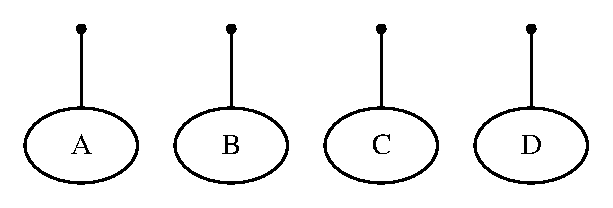
\includegraphics[width=0.44\textwidth]{List.eps}
%\caption{\label{fig:frog1}Hyperedge collection as list}


An odometer, hypergraph, and advancement function can represent all of the different programming and mathematical structures as both discrete points and functions to compute them. Collecting hyperedges from an odometer and advancement function until the function returns False is equivalent to exploring a $space$ in its entirety. Here the dimensions of the enumerated hyperedges are restricted to one expressing the enumeration of a vector.

\begin{lstlisting}
def OdometerAsList(hypergraph,odometer):
    if len(odometer) == 1:
        if odometer[0] + 1 < len(hypergraph):
            odometer[0] += 1
            return True
    return False

def EnumerateOdometer(hypergraph,odometer,func):
    returnValue = [ getHyperEdge(hypergraph,odometer) ]
    while func(hypergraph,odometer):
        returnValue.append( getHyperEdge(hypergraph,odometer))
    return returnValue

hypergraph = makeHyperGraph(sorted("ABCD"))
odometer = [0]
func = OdometerAsList
hyperedges_as_list = EnumerateOdometer(hypergraph,odometer,func)
\end{lstlisting}

Sorting a list is now equivalent to finding the correct odometer encoding ex- pressing the enumeration of the hypergraph as a sorted list. A function which advances the odometer from the current object to the next largest object which takes $N$ enumerations is equal in representation as an odometer of length $N$ where the next index contains the index of the node in the hypergraph which is next in the sort order. Interpretation depends upon the meta-context of the program using the hypergraph.
\newpage

